\documentclass[a4paper,english,helvetica,nologo,openbib,totpages]{europecv}
\usepackage[english]{babel} % This is mandatory
\usepackage[margin=1.8cm]{geometry}
\usepackage[hidelinks,unicode]{hyperref}
\usepackage{graphicx}
\usepackage{enumitem}

\makeatletter%
\renewcommand*\ecvtitle{%taken from definition file ecven.def and adapted to requirement
    \ecv@utf{\Large\textbf{C\ecv@kern u\ecv@kern r\ecv@kern r\ecv@kern
            i\ecv@kern c\ecv@kern u\ecv@kern l\ecv@kern u\ecv@kern m \ecv@kern V\ecv@kern
            i\ecv@kern t\ecv@kern a\ecv@kern e}}
}

\begin{document}

\pagestyle{empty}

% picture
\begin{minipage}{\textwidth}
  \raggedleft
  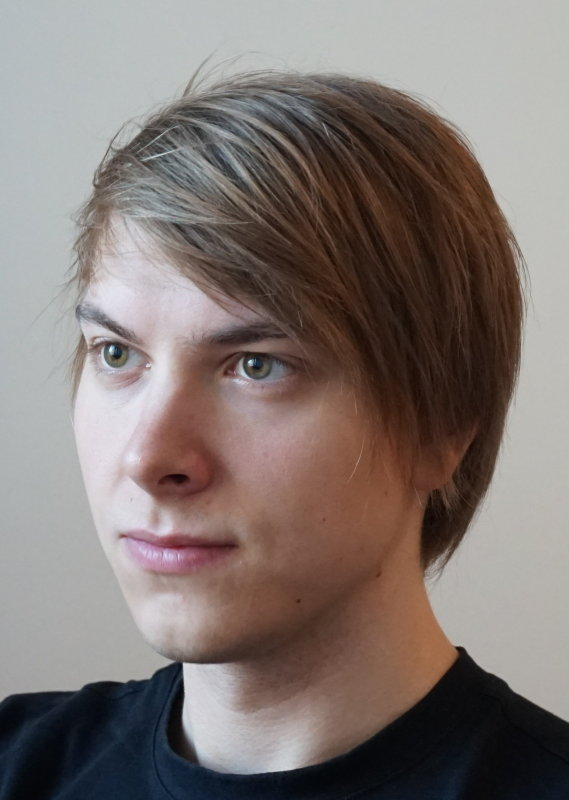
\includegraphics[height=7cm]{photo.jpg}
\end{minipage}
\vspace{-7.6cm}

\begin{europecv}

\vspace{0.5cm}

\ecvsection{Personal Information}
\ecvitem[5pt]{First name / Surname}{Tomáš Křížek}
\ecvitem[5pt]{Telephone}{+420 xxx xxx xxx}
\ecvitem[5pt]{E-mail}{\href{mailto:tomas.krizek@mailbox.org}{tomas.krizek@mailbox.org}}
\ecvitem[5pt]{Date of birth}{dd. mm. yyyy}
\ecvitem[5pt]{Permanent Address}{perm address}
\ecvitem[5pt]{\href{https://github.com/tomaskrizek}{GitHub}}{\url{https://github.com/tomaskrizek}}


\ecvsection{Work Experience}

\ecvitem{2018--present}{
\textbf{Research Software Engineer}\newline
\textit{CZ.NIC}
\begin{itemize}
  \item Working with low-level network protocols -- DNS, TLS, HTTP.
  \item Design \& development of DNS testing and benchmarking tools.
  \item Development of DNS resolver \& DNS-over-HTTPS functionality.
  \item Automation of CI testing \& maintenance of 10+ servers.
  \item Packaging software for Linux distributions (rpm, deb).
\end{itemize}
\textit{Python, C, Lua, Rust, git, DNS, Linux, Ansible, Bash, Docker}
\newline}

\ecvitem{2016--2017}{
\textbf{Associate Software Engineer}\newline
\textit{Red Hat}
\begin{itemize}
  \item Development of identity management solution.
  \item Design \& development of test automation framework.
  \item Packaging software for Linux distributions (rpm).
\end{itemize}
\textit{Python, Linux, git, Ansible, Bash, Docker, DNS, C}
\newline}

\ecvitem{2015--2016}{
\textbf{Python Developer}\newline
\textit{Technical University of Liberec}
\begin{itemize}
  \item Design \& development of multi-platform desktop application.
\end{itemize}
\textit{Python, git, Linux}
\newline}


\ecvsection{Education \& Training}

\ecvitem[8pt]
{2014--2016}{
\textbf{Master's degree} \textit{(cum laude)}, Information Technology\newline
\textit{Technical University of Liberec, Czech Republic}}

\ecvitem[8pt]
{2011--2014}{
\textbf{Bachelor's degree} \textit{(cum laude)}, Information Technology\newline
\textit{Technical University of Liberec, Czech Republic}}

\ecvitem[6pt]{2011}{
CCNA Exploration: Network Fundamentals\newline
\textit{Cisco Networking Academy}}
\ecvitem[6pt]{2010}{
IT Essentials: PC Hardware and Software\newline
\textit{Cisco Networking Academy}}

\clearpage

\ecvsection{Skills \& Technologies}
\ecvitem{\textit{Scripting Languages}}{}
\ecvitem{\textbf{Python}}{8+ years of experience}
\ecvitem{Bash}{6 years of experience}
\ecvitem[12pt]{Lua/LuaJIT}{4 years of experience}

\ecvitem{\textit{Compiled Languages}}{}
\ecvitem{\textbf{Rust}}{1 year of experience}
\ecvitem[12pt]{C}{5 years of experience}

\ecvitem{\textit{Automation \& CI}}{}
\ecvitem{Docker}{6 years of experience}
\ecvitem{Ansible}{5 years of experience}
\ecvitem[12pt]{Gitlab CI}{4 years of experience}

\ecvitem{\textit{Other}}{}
\ecvitem{Linux}{10+ years of experience}
\ecvitem{git}{10+ years of experience}


\ecvsection{Open-source contributions}

\ecvitem{
\href{https://gitlab.nic.cz/knot/knot-resolver}{Knot Resolver}}{
\textit{C \& Lua}\hfill
\url{https://gitlab.nic.cz/knot/knot-resolver}}

\ecvitem{\href{https://gitlab.nic.cz/knot/respdiff}{respdiff}}{
\textit{Python}\hfill
\url{https://gitlab.nic.cz/knot/respdiff}}

\ecvitem{\href{https://gitlab.nic.cz/knot/respdiff-rs}{respdiff-rs}}{
\textit{Rust}\hfill
\url{https://gitlab.nic.cz/knot/respdiff-rs}}

\ecvitem{\href{https://gitlab.nic.cz/knot/shotgun}{DNS Shotgun}}{
\textit{Python \& Lua \& C}\hfill
\url{https://gitlab.nic.cz/knot/shotgun}}

\ecvitem{\href{https://github.com/DNS-OARC/dnsjit}{dnsjit}}{
\textit{C \& Lua}\hfill
\url{https://github.com/DNS-OARC/dnsjit}}

\ecvitem{\href{https://gitlab.nic.cz/knot/resolver-benchmarking}{resolver-benchmarking}}{
\textit{Ansible \& Bash}\hfill
\url{https://gitlab.nic.cz/knot/resolver-benchmarking}}

\ecvitem{\href{https://github.com/NLnetlabs/domain}{domain}}{
\textit{Rust}\hfill
\url{https://github.com/NLnetlabs/domain}}

\ecvitem{\href{https://github.com/tomaskrizek/websharecli}{websharecli}}{
\textit{Python}\hfill
\url{https://github.com/tomaskrizek/websharecli}}

\ecvitem{\href{https://pagure.io/freeipa}{FreeIPA}}{
\textit{Python}\hfill
\url{https://pagure.io/freeipa}}

\ecvitem{\href{https://src.fedoraproject.org/user/tkrizek}{Fedora}}{
\textit{rpm packaging}\hfill
\url{https://src.fedoraproject.org/user/tkrizek}}

\ecvitem{\href{https://gitlab.nic.cz/labs/lxc-gitlab-runner}{lxc-gitlab-runner}}{
\textit{Ansible \& Bash}\hfill
\url{https://gitlab.nic.cz/labs/lxc-gitlab-runner}}

\ecvitem{\href{https://github.com/GeoMop/GeoMop}{GeoMop}}{
\textit{Python}\hfill
\url{https://github.com/GeoMop/GeoMop}}

\ecvitem{\href{https://gitlab.nic.cz/knot/deckard/}{deckard}}{
\textit{Python}\hfill
\url{https://gitlab.nic.cz/knot/deckard/}}


\ecvsection{About me}

\ecvitem{}{
I'm a backend software engineer and I enjoy working with protocols. My language
of choice for rapid development and prototyping is Python, which I have been
using for years.
\smallskip

When performance is valued over development speed, I'm not afraid to use a
low-level language. I've used C in the past, but after discovering Rust, I
believe it has much better tradeoff between development time and runtime
performance, even tough my experience with Rust is limited.
\smallskip

I prefer to work with free and open-source projects. I'm a long time Linux user
and I'm familiar with all the major distributions.
}

\end{europecv}

\end{document}
